\chapter{CodeWarrior for MCU}

Prin intermediul utilitarului \textit{CodeWarrior} se pune la dispoziție un mediu complet de dezvoltare software pentru sistemele embedded. Cu ajutorul acestei suite puse la dispoziție de Freescale, se oferă un suport consistent în ceea ce privește dezvoltarea aplicației (inclusiv partea de depanare a ei) reducându-se timpul și efortul necesar programării unui dispozitiv embedded. CodeWarrior se bazează pe Eclipse și conține mai multe componente. În primul rând are inclus un sistem de build, un compiler și un debugger engine. Pentru utilizarea lui este necesară o licență. În cazul ședințelor tehnice ce vor avea loc, pe parcursul acestui concurs, veți beneficia de toate condițiile necesare utilizării cu succes al acestui utilitar.

De aproximativ un an de zile, Freescale a introdus și un tool similar pentru familia \textit{Kinetis} și anume \textit{Kinetis Design Studio} ce înglobează o serie de module open-source. Este soluția perfectă cu care puteți să continuați să dezvoltați propriile aplicații embedded după terminarea acestui concurs. În continuare, vom prezenta \textit{CodeWarrior} ca și tool pe care îl vom folosi, dar să știți că o dată ce v-ați familarizat cu acesta din urmă, o să fie la îndemână și experimentarea pe alte soluții - gen \textit{Kinetis Design Studio}.

Pentru programarea unui microcontroller se pot folosi diverse metode, dintre care programarea bazată pe interfaţa serială, folosirea unui programator ISP (\textit{In-System Programming}) ce foloseşte interfaţa serială SPI sau folosirea unui \textit{bootloader}. În cadrul acestui concurs vom folosi ultima variantă, un bootloader fiind un program încărcat la sfârşitul memoriei program a microcontroller-ului (de exemplu programat folosind un programator ISP). Execuţia codului încărcat astfel va începe din zona de boot.

\section{Programarea microcontroller-ului folosind OpenSDA}

OpenSDA este un firmware ce rulează pe un core independent, și anume un K20DX (produs tot de Freescale) și care pune la dispoziție bootloader-ul de care avem nevoie pentru a putea programa microcontroller-ul. Acest firmware se poate descărca de la adresa\footnote{\myhref{http://www.pemicro.com/opensda/}{http://www.pemicro.com/opensda/}}, el necesitând și programarea sa pe placă. Bineînțeles, în cazul plăcilor de dezvoltare pe care vi le punem la dispoziție, vom realiza noi această parte, plăcile având deja ultima versiune a firmware OpenSDA. Totuși dorim să vă prezentăm în continuare și cum puteți face acest lucru voi înșiși acasă. Pașii pe care trebuie să îi urmați ar fi următorii:

\begin{wrapfigure}{r}{0.4\textwidth}
    \vspace{-25pt}
    \center{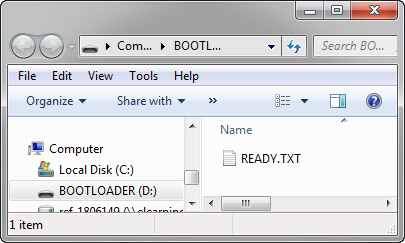
\includegraphics[width=0.4 \textwidth]{images/OSDevice.png}}
    \vspace{-20pt}
    \caption{\label{fig:CodeWarrior-OSDevice} Accesarea modului Bootloader}
    \vspace{-25pt}
\end{wrapfigure}

\begin{enumerate}
    \item Primul pas constă în intrarea în modulul \textit{Bootloader}, prin apăsarea butonului de \textit{Reset} în timp ce placa este alimentată de la sursă de tensiune. Mare atenție, pentru că alimentarea plăcii trebuie să se facă în timp ce acest buton este ținut apăsat.
    \item Confirmarea hardware pentru faptul că totul este bine și sunteți în acest mod, este oferită de un led verde ce se află lângă modulul OpenSDA de pe Freedom board.
    \item În acest moment, dacă vă conectați calculatorul personal cu un cablu USB la Freedom board, sistemul de operare ar trebui să vă recunoască un nou device în sistem, așa cum este ilustrat în figura \ref{fig:CodeWarrior-OSDevice}.
    \item Folosind o simplă operație de tip drag \& drop se pot copia fișierele cu extensia SDA (ce au fost descărcate anterior) în cadrul device-ul ce se află în modul Bootloader. Procesul este asemănător cu cel al copierii unui fișier de pe o partiție pe alta.
    \item Un alt reset al plăcii (prin deconectarea și reconectarea la o sursă de alimentare) va produce începerea rulării fișierelor SDA încărcate la pasul anterior.
\end{enumerate}

După ce ați urmat toți pașii de mai sus, veți putea utiliza CodeWarrior fără probleme în programarea și depanarea programelor voastre. Aveți totuși grijă să creați un proiect având stabilită ca și conexiunea OpenSDA (și nu Segger, spre exemplu) pentru a-i putea specifica tool-ului modul de programare. Altfel, riscați să nu puteți programa placa!

Ajunși în acest punct, putem să începem să ne obișnuim cu mediul de dezvoltare și mai ales interfața pe care o oferă. Ați mai utilizat un IDE (\textit{Integrated Development Environment}) până acum?

\section{Vedere de ansamblu asupra utilitarului}

Figura \ref{fig:CodeWarrior-VedereDeAnsamblu} (de pe pagina următoare) ilustrează cele mai importante ferestre din mediul de dezvoltare \textit{CodeWarrior for MCU}. În partea de sus avem meniuri și butoane pentru acces rapid la anumite funcționalități, în stânga avem detalii legate de proiectele create și fișierele asociate lor, în centru ecranului apare un editor prin care se poate modifica conținutul fișierelor unui proiect, iar în partea de jos se poate observa dacă proiectul nostru conține erori. Acestea ar fi în mare câteva din elementele pe care le vom folosi, utilitarul punând la dispoziție o multitudine de feature-uri.

În cele ce urmează vor fi prezentate succint câteva dintre acțiunile cele mai des întâlnite pe care le veți realiza pe parcursul dezvoltării programului vostru.

\begin{figure}[h!]
    \vspace{-15pt}
    \center{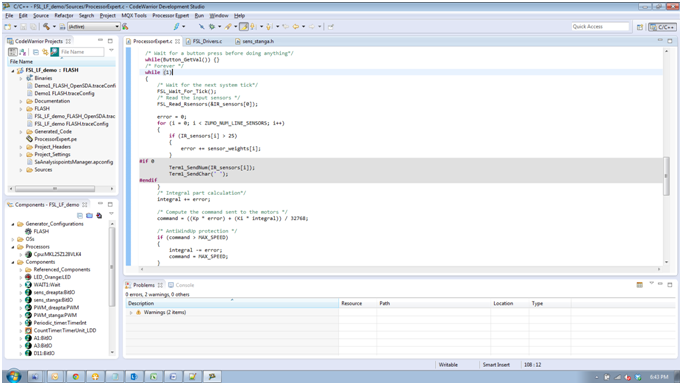
\includegraphics[width=1.0 \textwidth]{images/CodeWarriorMCU.png}}
    \vspace{-20pt}
    \caption{\label{fig:CodeWarrior-VedereDeAnsamblu} CodeWarrior for MCU - Vedere de ansamblu}
    \vspace{-10pt}
\end{figure}

\section{Compilarea proiectului}

\begin{wrapfigure}{r}{0.5\textwidth}
    \vspace{-50pt}
    \center{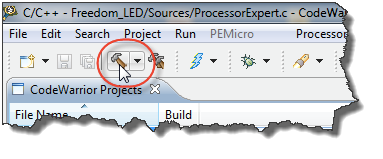
\includegraphics[width=0.5 \textwidth]{images/BuildProject.png}}
    \vspace{-30pt}
    \caption{\label{fig:CodeWarrior-CompilareProiect} Cum se poate compila proiectul}
    \vspace{-10pt}
\end{wrapfigure}

Pentru a compila proiectul, după ce în prealabil s-a generat codul folosind ProcessorExpert (despre acest utilitar veți afla mai multe în capitolul ~\textit{\nameref{sec:ProcessorExpert}}) și voi v-ați scris codul vostru sursă, puteti folosi butonul din figura \ref{fig:CodeWarrior-CompilareProiect} sau de ce nu puteți folosi meniul principal și anume opțiunea \textit{Project $\rightarrow$ Build Project}. Indiferent de varianta aleasă rezultatul va fi același.

\begin{wrapfigure}{l}{0.5\textwidth}
    \vspace{-20pt}
    \center{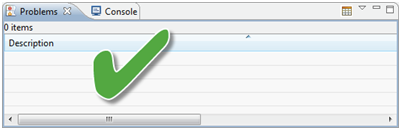
\includegraphics[width=0.5 \textwidth]{images/ProblemsView.png}}
    \vspace{-20pt}
    \caption{\label{fig:CodeWarrior-FereastraProblems} Când totul decurge bine...}
    \vspace{-10pt}
\end{wrapfigure}

Dacă totul a decurs cu bine, trebuie să nu avem erori în fereastra \textit{"Problems"}, așa cum evidențiază figura \ref{fig:CodeWarrior-FereastraProblems}. Această fereastră poate conține atât erori cât și warning-uri. Chiar dacă warning-urile nu împiedică procesul de building așa cum o fac erorile, este indicat să le luați în seamă pentru că ele pot evidenția alte probleme, ce apar la runtime (la rularea codului de pe placă).

\newpage

\section{Descărcarea codului pe placă}

\begin{wrapfigure}{r}{0.7\textwidth}
    \vspace{-25pt}
    \center{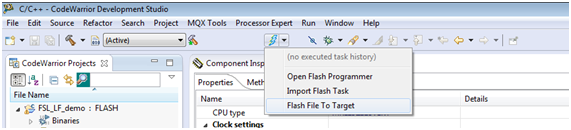
\includegraphics[width=0.7 \textwidth]{images/FlashProgrammer1.png}}
    \vspace{-20pt}
    \caption{\label{fig:CodeWarrior-FlashProgrammer1} Încărcarea codului pe placă}
    \vspace{-20pt}
\end{wrapfigure}

În urma compilării rezultă un executabil ce va trebui să fie flash-uit pe robot. Acest proces este realizat cu ajutorul unui instrument numit \textit{Flash Programmer}, iar figurile \ref{fig:CodeWarrior-FlashProgrammer1} și \ref{fig:CodeWarrior-FlashProgrammer2} vin să explice pașii ce trebuie urmăriți. Partea cea mai frumoasă o constituie faptul că aceste configurări vor fi făcute o singură dată. Ele sunt salvate local și pot fi refolosite de fiecare dată când este nevoie de ele.

\begin{wrapfigure}{r}{0.5\textwidth}
    \vspace{-70pt}
    \center{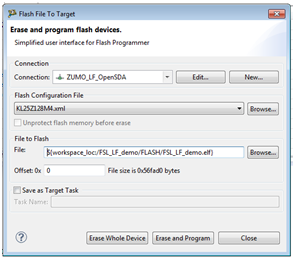
\includegraphics[width=0.5 \textwidth]{images/FlashProgrammer2.png}}
    \vspace{-20pt}
    \caption{\label{fig:CodeWarrior-FlashProgrammer2} Flash-uirea unui executabil}
    \vspace{-20pt}
\end{wrapfigure}

\section{Debugging}

Până să ajungeți la o versiune funcțională, pe care să o puteți prezenta la concurs sau în cercul vostru de prieteni, va fi ceva de munca. Lucrurile vor fi abordate pas cu pas, va trebui de multe ori să faceți un debugging avansat pentru a înțelege ce e greșit în algoritmul vostru de robotul nu face ceea ce doriți voi să facă. În cazul în care vreți să puteți executa programul în modul debug (pas-cu-pas), puteți folosi butonul exemplificat în figura \ref{fig:CodeWarrior-Debugging}. Nu uitați, pentru a folosi acest mod, robotul trebuie să rămână conectat la laptop printr-un cablu. Ca alternativa - recomandată, de altfel – puteți folosi interfața serială pentru a trimite date dinspre robot spre laptop (mai multe detalii despre această interfață puteți citi la capitolul \textit{~\nameref{sec:InterfataSeriala}})

\begin{wrapfigure}{l}{0.5\textwidth}
    \vspace{-20pt}
    \center{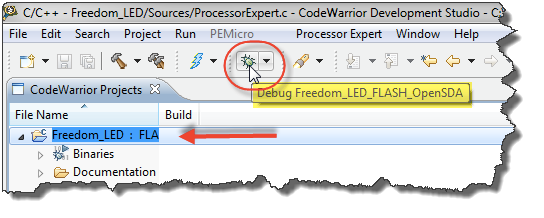
\includegraphics[width=0.5 \textwidth]{images/Debugging.png}}
    \vspace{-25pt}
    \caption{\label{fig:CodeWarrior-Debugging} Accesarea modului de debugging}
    \vspace{-20pt}
\end{wrapfigure}

Folosirea acestei interfețe seriale, vă va permite să faceți debugging folosind apeluri ale funcției \textit{printf}, cea mai primitivă metodă de a depana un program software. Din fericire, există și alte metode ceva mai avansate, cu rezultate mult mai bune, metode ce vor fi prezentate la ședințele tehnice.

\section{Processor Expert}

Processor Expert este un sistem de dezvoltare pus la dispoziție de firma \textit{Freescale Semiconductor} ce vine o dată cu utilitarul \textit{CodeWarrior for MCU}, prin intermediul căruia se pot crea și configura componente software ce generează cod sursă pentru microcontrollere produse de \textit{Freescale}. O astfel de componentă poate fi un driver (adică un soft ce asigură interacțiunea cu o unitatea hardware), un algoritm sau o colecție de funcții software ce deservesc un obiectiv. O componentă poate fi, de exemplu, un driver ce permite accesul facil la pinii de intrare / ieșire puși la dispoziție de un microcontroller.

Folosirea Processor Expert înleșneste lucrul cu platforma hardware prin abstractizarea detaliilor de la nivelul low-level. Putem spune că avem de-a face cu o programare vizuală, în care este mai mult folosit mouse-ul decât tastatura. Noi, ca și programatori, vom avea mai multe setări și opțiuni de configurat pentru respectivul modul, pentru ca mai apoi, codul să fie generat automat în funcție de inputul pe care l-am specificat. 

În cadrul acestui concurs, vom folosi Processor Expert. De ce? Răspunsul este foarte simplu. Cu ajutorul lui putem adăuga și configura componente, apoi genera cod sursă C pentru aceste componente. Pornind de la codul generat de Processor Expert, voi trebuie să adăugați cod scris de voi pentru a implementa algoritmii care să conduca și să ajute robotul să urmărească linia.

\subsection{Accesarea utilitarului}

\begin{wrapfigure}{r}{0.3\textwidth}
    \vspace{-60pt}
    \center{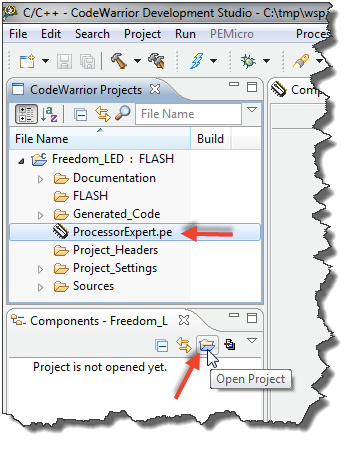
\includegraphics[width=0.3 \textwidth]{images/ProcessorExpert.png}}
    \vspace{-25pt}
    \caption{\label{fig:CodeWarrior-ProcessorExpert} Accesarea componentelor Processor Expert}
    \vspace{-50pt}
\end{wrapfigure}

După deschiderea proiectului în \textit{CodeWarrior for MCU}, în cazul în care fereastra \textit{Processor Expert} nu este vizibilă, va trebui să procedăm ca în figura \ref{fig:CodeWarrior-ProcessorExpert}.

\subsection{Adăugarea unei noi componente}

\begin{wrapfigure}{r}{0.3\textwidth}
    \vspace{-30pt}
    \center{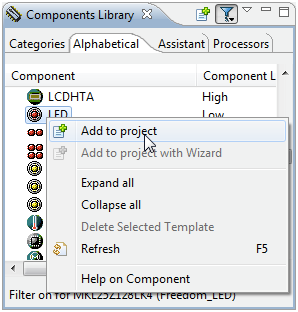
\includegraphics[width=0.3 \textwidth]{images/ProcessorExpertAdd.png}}
    \vspace{-20pt}
    \caption{\label{fig:CodeWarrior-ProcessorExpertAdd} Cum se adaugă o nouă componentă?}
    \vspace{-10pt}
\end{wrapfigure}

Înainte de a putea utiliza o componentă definită de acest utilitar, va trebui mai întâi, așa cum este și logic, să o adăugăm în cadrul proiectului nostru. Procesul de adăugare a unei componente este relativ simplu, fiind similar cu cel descris în figura \ref{fig:CodeWarrior-ProcessorExpertAdd}, din cadrul fereastrei de lucru \textit{Components Library}.

\subsection{Generarea de cod sursă}

După ce toate componentele necesare au fost adăugate și setate corect (sau după modificarea setărilor unor componente) trebuie lansată o comandă prin care Processor Expert va fi înstiințat de faptul că trebuie să genereze codul sursă pentru componentele existente în proiect. Acest proces de înștiințare are loc doar prin apăsarea unui singur buton și anume - \textit{"Generate Processor Expert Code"}. După apăsarea butonului, utilitarul vă va ruga să aveți răbdare...

\textcolor{red}{Notă:} Codul generat de Processor Expert conține zone ca cele de mai jos, rezervate special pentru codul pe care voi îl veți scrie. Nu încercați să modificați sau să scrieți cod în afara acestor zone, deoarece o noua generare a codului Processor Expert vă va șterge tot ce ați adăugat. Iar asta nu este foarte plăcut, pentru că va trebui să o luați de la capăt cu acele modificări manuale.

\newpage

\begin{figure}[h!]
    \vspace{-10pt}
    \center{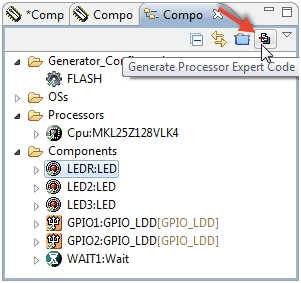
\includegraphics[width=0.3 \textwidth]{images/ProcessorExpertGenerate.png}}
    \vspace{-10pt}
    \caption{\label{fig:CodeWarrior-ProcessorExpertGenerate} Generarea de cod în Processor Expert}
    \vspace{-10pt}
\end{figure}

\lstinputlisting[caption=Inițializarea modulelor hardware, style=customc]{sources/generatingPExCode.lst}